\documentclass[a4paper]{report}
\usepackage[utf8]{inputenc}
\usepackage{amssymb}
\usepackage{amsmath}
\usepackage{amsthm} 
\usepackage{url}
\usepackage{xspace}
\usepackage{graphicx}
\usepackage[vlined]{algorithm2e} % lib for pseudo code
\usepackage{float}  % lib for pseudo code
\usepackage[T1]{fontenc}
\usepackage{pgfplots}
\usepackage{caption}
\usepackage{subcaption}
\usepackage{array}
\usepackage{mdframed}
\usepackage{rotating}
\usepackage{multirow}
\usepackage{dirtytalk}
\usepackage{longtable}
\usepackage[titletoc]{appendix}
\usepackage{hyperref}

\usepackage{listings}
\usepackage{color}

%New colors defined below
\definecolor{codegreen}{rgb}{0,0.6,0}
\definecolor{codegray}{rgb}{0.5,0.5,0.5}
\definecolor{codepurple}{rgb}{0.58,0,0.82}
\definecolor{backcolour}{rgb}{0.95,0.95,0.92}
\definecolor{lightgray}{rgb}{.9,.9,.9}
\definecolor{darkgray}{rgb}{.4,.4,.4}
\definecolor{purple}{rgb}{0.65, 0.12, 0.82}

\lstdefinelanguage{JavaScript}{
  keywords={typeof, new, true, false, catch, function, return, null, catch, switch, var, if, in, while, do, else, case, break},
  keywordstyle=\color{blue}\bfseries,
  ndkeywords={class, export, boolean, throw, implements, import, this},
  ndkeywordstyle=\color{darkgray}\bfseries,
  identifierstyle=\color{black},
  sensitive=false,
  comment=[l]{//},
  morecomment=[s]{/*}{*/},
  commentstyle=\color{purple}\ttfamily,
  stringstyle=\color{red}\ttfamily,
  morestring=[b]',
  morestring=[b]"
}

%Code listing style named "mystyle"
\lstdefinestyle{mystyle}{
  backgroundcolor=\color{backcolour},   commentstyle=\color{codegreen},
  keywordstyle=\color{magenta},
  numberstyle=\tiny\color{codegray},
  stringstyle=\color{codepurple},
  basicstyle=\footnotesize,
  breakatwhitespace=false,         
  breaklines=true,                 
  captionpos=b,                    
  keepspaces=true,                 
  numbers=left,                    
  numbersep=5pt,                  
  showspaces=false,                
  showstringspaces=false,
  showtabs=false,                  
  tabsize=2
}

%"mystyle" code listing set
\lstset{style=mystyle}


%Setup of the TableOfContent to incl. subsubsection
\setcounter{tocdepth}{3}
\setcounter{secnumdepth}{3}

\RestyleAlgo{boxruled}
\LinesNumbered


\newcolumntype{L}[1]{>{\raggedright\let\newline\\\arraybackslash\hspace{0pt}}m{#1}}

\graphicspath{ {Graphics/Images/} }

\usepackage{newunicodechar}
\newunicodechar{∙}{\cdotp}

\newcommand{\parahead}[1]{{\vspace*{6pt}\noindent\textbf{#1}\xspace\xspace\xspace\xspace}}

\newcommand{\heading}[1]{{\vspace{6pt}\noindent\sc{#1}}}

% Command for making <--> arrow with text above
\makeatletter
\newcommand\xleftrightarrow[2][]{%
  \ext@arrow 9999{\longleftrightarrowfill@}{#1}{#2}}
\newcommand\longleftrightarrowfill@{%
  \arrowfill@\leftarrow\relbar\rightarrow}
\makeatother

\newcommand{\dotp}[2]{\ensuremath{\left\langle {#1},{#2}\right\rangle}\xspace}
\newcommand{\Z}{\ensuremath{\mathbb{Z}}\xspace}
\newcommand{\Zq}{\ensuremath{\Z_q}\xspace}
\newcommand{\ZqStar}{\ensuremath{\Z_q^*}\xspace}
\newcommand{\Zp}{\ensuremath{\mathbb{Z}_p}\xspace}

\def\polyfactor{n\, \log_2^2 n}
\newcommand{\bigO}[1]{\ensuremath{\mathcal{O}\left(#1\right)}\xspace}
\renewcommand{\O}[1]{\ensuremath{{\mathcal{O}\left(#1\right)}}\xspace}


\theoremstyle{plain}
\newtheorem{thm}{Theorem}[subsection]
\newtheorem{lemma}{Lemma}[subsection]

\mdfdefinestyle{defstyle}{frametitlerule=true, frametitlerulewidth=0px}
\mdtheorem[style=defstyle]{defi}{Definition}[subsection]

\mdtheorem[style=defstyle]{infobox}{}[subsection]

\begin{document}

%***************************************************************
%               Title Page
%***************************************************************
\begin{titlepage}

\newcommand{\HRule}{\rule{\linewidth}{0.5mm}} % Defines a new command for the horizontal lines, change thickness here

\center % Center everything on the page
 
%----------------------------------------------------------------------------------------
%	HEADING SECTIONS
%----------------------------------------------------------------------------------------

\textsc{\LARGE Syddansk Universitet}\\[0.5cm] % Name of your university/college
\textsc{\large Software Engineering of Mobile Systems}\\[1.5cm] %Minor Heading 


%----------------------------------------------------------------------------------------
%	TITLE SECTION
%----------------------------------------------------------------------------------------

\HRule \\[0.4cm]
{ \huge \bfseries BikeBus}\\[0.4cm] % Title
\HRule \\[1.5cm]
 
%----------------------------------------------------------------------------------------
%	AUTHOR SECTION
%----------------------------------------------------------------------------------------

\begin{minipage}{0.4\textwidth}
\begin{flushleft} \large
\emph{Author:}\\
Sune Chung \textsc{Jepsen} % Your name
Admir \textsc{Muric}\\ % Your name
Anna \textsc{\o}lgaard \textsc{Nielsen} % Your name
\end{flushleft}
\end{minipage}
~
\begin{minipage}{0.4\textwidth}
\begin{flushright} \large
\emph{Supervisor:} \\
Mikkel Baun \textsc{Kjærgaard} % Supervisor's Name
\end{flushright}
\end{minipage}\\[2cm]

% If you don't want a supervisor, uncomment the two lines below and remove the section above
%\Large \emph{Author:}\\
%John \textsc{Smith}\\[3cm] % Your name

%----------------------------------------------------------------------------------------
%	DATE SECTION
%----------------------------------------------------------------------------------------

{\large September 2017}\\[2cm] % Date, change the \today to a set date if you want to be precise

%----------------------------------------------------------------------------------------
%	LOGO SECTION
%----------------------------------------------------------------------------------------

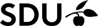
\includegraphics{SDU_logo.png}\\[.5cm] % Include a department/university logo - this will require the graphicx package
 
%----------------------------------------------------------------------------------------

\vfill % Fill the rest of the page with whitespace

\end{titlepage}
%\chapter*{Acknowledgements}
%
It has been a learning period for the past six months, where we have studied the public verifiable secret sharing protocol. It has been a steep learning curve, but as we have worked with the topics on  a theoretical and practical level, we have gained an understanding of the protocol and its application.\\

\noindent
We would like to express our gratitude to our supervisor Ignacio Cascudo for his guidance and expert knowledge on this area throughout our work with this Master thesis. 

%\chapter*{Summary}
%In this Master thesis we will study the public verifiable secret sharing protocol and how it can be used in an electronic voting application based on the work from \cite{Schoenmakers1999}. Based on this knowledge we will design and implement a web based electronic voting application.\\

\noindent
Our work with this protocol leads to the following main topics which should cover our objective about Shamirs secret sharing, multiparty computation, public verifiable secret sharing protocol and our implementation of an electronic voting application.

\begin{enumerate}
    \item Voting
    \item Mathematical understanding
    \item Multiparty computation
    \item Electronic voting protocol
    \item Designing the application
    \item The application
    \item Reflection
\end{enumerate}

\noindent
We start with describing the concepts of electronic voting and the challenges with the different types of electronic voting applications. We will use other studies and their demands for concrete security requirements, which we can include in our consideration for our electronic voting application.  \\

\noindent
To understand the public verifiable secret sharing protocol one need some basic mathematical understanding and some knowledge about cryptographic tools. Modular arithmetic and group theory will be key elements in understanding how the protocol works. Regarding to the cryptographic tools we will present the discrete logarithm problem which is the security primitive for this protocol.\\

\noindent
Multiparty computation is basically about allowing parties to compute some function on some private inputs, in such a way that they learn the result but not the inputs from the other parties. Secret sharing is about hiding information in a random polynomial. By using this polynomial, parties can create shares based on evaluations in the polynomial. If enough parties then collect their shares together they will be able to recover the secret.  We will present a simple secret sharing example which illustrate how a secret can be distributed and reconstructed. In addition to these properties the public verifiable secret sharing protocol gives us the ability to publicly verify the validity of the shares among the parties involved in this protocol. This means that the protocol is secure against malicious parties which try to send votes which they are not supposed to do. \\

\noindent
The part describing the electronic voting protocol is divided into two parts, a basic and a more-in-depth description of the protocol. The first part is intended to supply enough basic knowledge for a software developer to implement a simple voting application based on the protocol. The second part is intended to give a more thorough insight of the protocol, here we describe the mathematical justifications behind the protocol as well as the proofs to verify the correctness and the consistency of the protocol. \\


\noindent
Designing the application is about architectural strategies for our application based on the knowledge from literature of \cite{Bass} and \cite{Baerbak10}. We took the security requirements of electronic voting in general as described in \cite{Cet09} as the functional demands for our application. To extract the architectural demands, such as \textit{Interoperability}, \textit{Modifiability} and \textit{Testability}, we used Quality attribute scenarios which is a way of defining a clear architectural measurable demands. In order to illustrate the impact these demands have on the architecture we will use several documentation methods here among diagrams. The process of deriving these demands is done through an Quality attribute workshop \cite{BarbacciQualityAttribute2003}. Since we have limited time we only used the structure of the Quality attribute workshop for deriving the Quality attributes scenarios without actually holding a workshop. Furthermore the structure of the workshop helped us prioritize among a long list of demands, and helped us derive the most important scenarios which we then proceeded on implementing.\\


\noindent
In the application part, we will elaborate on how we have implemented the final design of the architecture on a proof-of-concept application. \\

\noindent
Lastly the reflection part, summarizes the most important reflections on our results from the theoretical and the practical parts of this thesis. 



  


 

\clearpage

\tableofcontents


%***************************************************************
%               Part 1: Introduction
%***************************************************************
\chapter{Introduction}
    % Admir
\section{Introduction}
\textcolor{red}{Motivation and Context: Describe the project’s motivation and the respective context right here. In this part, also include references to literature that provides extra arguments.}\\


Multiple studies have documented that psychical activities has a disease preventive effect. Other studies shows that psychical activity has a positive effect on people's learning ability regardless of their age [ref: Sundhedsstyrelsen/Kulturministeriets Udvalg for Idrætsforskning]. Therefor we need people to exercise more, and preferably start as young as possible. \\


In Denmark we have really strong biking traditions. We need to hold onto this biking culture and pass it on to our children so that they can get the same joy of biking. 


To improve the biking environment the government has initiated a "green" strategy which focuses on biking[\textcolor{red}{REF?}]. The bike is a cheap, healthy and a pollution-free vehicle. Other benefits could be fewer accidents and less noise. There is a need for initiatives and innovation that promote the joy of continuous use of biking. \\


Odense is the city of biking. In 2015 Odense received a price for best biking city[\textcolor{red}{REF?}]. Biking is highly prioritized in the city infrastructure. Different bike paths and bridges have been constructed over the past years. In different places in the city there are sensor stations where specialized software can register cyclists through sensors. 


We need to make it more attractive and easier to choose the bike for work or school etc. We can do this by creating better bike paths, fewer stops, secure biking parking spaces and new bike facilities. Another strategy is to make it fun to use the bike every morning by either competing or collaborating with friends. \\


One initiative is the concept CykelScore, which main idea is to encourage mainly children to bike in the city by using gamification. CykelScore has put up multiple bike stations around the city containing a chip to register whenever a cyclist passes by. Every time a cyclist passes a CykelScore station they get a point, and they can collect all their points in a mobile application and compete with their friends. \\


This leads to a core observation namely how we as software engineering's can exploit software which encourage and motivate the use of biking and thereby support the many reasons for biking and doing psychical activity at the same time. 
Our project focuses on how friends can collaborate and help each other use the bike more by creating "Bike Busses".
    
    \section{Motivation} It could be interesting to create a mobile application combined with theoretical knowledge on mobile systems and methods for engineering mobile systems. Based on the CykelScore concept our focus will be on increasing the safety of biking by using mobile sensing to coordinate “Biking Buses” for younger kids supervised by older kids.   \\


 In this solution we will have focus on designing a flexible architecture. Using known software design principle from \cite{Bass} and \cite{Baerbak10}, we discuss and reflect on different solutions.
 
 
 %**************************************Definition Software engineering
\begin{defi}[\textbf{Software engineering}]
Concerned with developing and maintaining software systems that behave reliably and efficiently, are affordable to develop and maintain,
and satisfy all the requirements that customers have defined for them. [ACM]
\end{defi}
%**************************************Definition Software engineering End


 %**************************************Definition Mobile systems
\begin{defi}[\textbf{Mobile systems}]
% Admir
Mobile systems covers software systems that run on computers that are expected to be transported during normal usage. Systems depend on innovations in mobile
communications and mobile hardware.
\end{defi}
%**************************************Definition Mobile systems End


 %**************************************Definition Mobile systems
\begin{defi}[\textbf{Mobile sensing}]
Mobile sensing is the use of mobile devices for sensing and learning physical and social phenomenon and using such information for
informing, sharing and persuasion among humans.
\end{defi}
%**************************************Definition Mobile systems End



    
    % Admir
\section{Objectives}
\textcolor{red}{Problem and Objective: What is the (exact) problem to be addressed/solved with the application you build. Note, describe the problem and the overall objective only.}\\


\iffalse
\noindent
What we should address:
\begin{enumerate}
    \item  Analyze architectural structures and qualities of a mobile system and provide arguments for what needs to be done to evolve the architecture according to new and changing requirements
            
    \item  Explain the code base in a larger mobile system and explain how incremental expansions of functionality can be made according to changing requirements
    
    \item   Provide arguments for the choice of technologies in a given mobile system project taking into account the architectural and project requirements
    
    \item Provide arguments for how to architect mobile system solutions that address energy efficiency and resource availability challenges. 
\end{enumerate}
\fi

This project consists of two main parts. The first a theoretical background where we study the concepts behind mobile sensing. In the second part, we will describe our process for designing the bikingbus mobile application. Basically this project have the following objectives. 

\begin{enumerate}
    \item   Describe the theory behind different aspect of mobile sensing. The aim is to understanding the concept behind a mobile sensing application and what one needs to handle. 
            
    \item  Analyze requirements, design and prototype a mobile bikebus application with focus on the architectural design. From the requirements we shall address energy efficiency and resource availability. Known software design principles will be used to acquire high flexibility software quality to assist incremental changes in the demands. 

\end{enumerate}



    
    % Sune

\section{Limitations}

The following limitations have be identified.

\begin{itemize}
    \item Working in depth  with  both practice and the theory.

\end{itemize}



    
    % Admir
\section{Report outline} \textcolor{red}{Provide some information, where to find what in the report.}


\begin{enumerate}
    \item Theoretical for Mobile sensing
    \begin{enumerate}
        \item Mobile sensing
        \item Challenges regards to inform, Share, Persuasion and what can we learn from other mobile sensing systems.
        \item Spatial data
        \item Human Behavior regoniction
    \end{enumerate}
    \item Design of application
    \begin{enumerate}
        \item QAS, architectural challenges mobile systems
        \item Architectural prototyping
        \item Tactics resource adaptability and energy efficiency
        \item Performence testing
        \item Software implementation and results
    \end{enumerate}
    \item Reflection and Discussion
\end{enumerate}

%***************************************************************
%               Part 1: Mobile sensing
%***************************************************************
\chapter{Mobile Sensing} 
    % Admir
\section{Types of mobile sensing}  
% TODO: 
% Apply definitions
% Explain difference between participatory and opportunistic sensing
% Relate to articles.
% Relate to app (start geofence -> continuous sensing -> end geofence)
% Reflect and discuss. 


%**************************************Definition Software 
\begin{defi}[\textbf{Participatory Sensing}]
Participatory  Sensing  emphasizes  the  involvement  of  citizens  and  community  groups  in  the 
process  of  sensing  and  documenting  life  where  they  live,  work,  and  play. \cite{Goldman2009}. 
\end{defi}
% https://www.researchgate.net/publication/42831772_Participatory_Sensing_A_Citizen-Powered_Approach_to_Illuminating_the_Patterns_that_Shape_our_World

\begin{defi}[\textbf{Opportunistic Sensing}]
Opportunistic sensing shifts the burden of supporting an application from the custodian to the sensing system, automatically determining when devices can be used to meet application requests. \cite{Lane:2008:USS:1411759.1411763} 
\end{defi}



\begin{enumerate}
    \item  Participatory sensing
    
    \begin{enumerate}
        \item  User actively engages in the data collection activity

        \item  Manually determines how, when, what, and where to sample
   
    \end{enumerate}
            
    \item  Opportunistic sensing
    
        \begin{enumerate}
        \item   Data collection runs as a continuous background activity

    \end{enumerate}
\end{enumerate}

\section{Application Types}
% TODO: 
% Apply definitions
% Explain difference between indivudual, group and community
% Relate to articles.
% Relate to app 
%   - App is individual (now)
% Reflect and discuss. 
%   - Group could be used for sensing (location)
%     precision/accurarcy (future)
%   - Community could be to provide route data for 
%     municipality (future)
    \begin{enumerate}
        \item  Individual activity sensing fitness applications, behavioural suggestions

        \item  Group activity sensing groups to sense common activities and help achieving group goals. Eg: assess neighbourhood safety, collective recycling efforts 
        
        \item Community sensing large scale sensing, where a large number of people have the same application installed. E.g., tracking spread of disease across a city, congestion in a city.
    \end{enumerate}
    
\section{Context Awareness}
% TODO:
% Apply definitions
% Explain context awareness, classification and phone context
% Give example of how to combine multiple sensors
%   - ex: gyroscope and accelerometer
% Relate to articles
% Relate to app: how we use classification
% Reflect and discuss. Can context awareness be used in other ways in our app?

% Relate to activity recognition (uses accelerometer


    
\chapter{Sensor Challenges}
    % Anna og Sune (3.2)

%TODO:
% Introduction to data collection, data processing and closing the sensing loop


\section{Data Collection}
% TODO: 
% Apply definitions
% Little introduction
% Tactics:
%    - Part into intervals
%    - Sampling rate
%    - Combinations of sensors (location/gps + 
%      accelerometer + gyroscope)
% Relate to articles
% Relate to app
% Reflect and discuss

The first part of continuous sensing is the data collection. In this section the data collection process of our application will be described along with ideas for extension.
Data collection needs to deal with the concepts of sensor choice, sampling rate and phone context, which can be determined using a tactic of a defined quality attribute. When developing on a mobile device the energy efficiency tactics will most likely be applied, since the battery life is a very valuable asset.  

The data collection from continuous sensing in our application consists of: 
\begin{itemize}
    \item Location data - GPS sensor (Fine Location)
    \item Activity Recognition data from Google API - Low-power Sensors \cite{androidActivity}
\end{itemize}

Location data uses the fine location sensor to determine the actual path of the bike route when a bikebus has startet. To determine when a bikebus has startet and ended the notion of "Geofencing" is used to trigger when the user is inside a radius of \textcolor{red}{<<INSERT RADIUS>>}. 
When a geofence event has been raised some constraints must be fulfilled before the continuous data collection can begin.
\begin{itemize}
    \item The current timestamp must be within the time window textcolor{red}{<<INSERT TIME WINDOW>>} of an enlisted bikebus
    \item The current activity must be of type "ON\_BICYCLE"
\end{itemize}
Once the constraints have been fulfilled the data collection begins \textcolor{red}{<<INSERT SENSING TACTIC>>} by collecting locations at the sample rate of \textcolor{red}{<<INSERT SAMPLE RATE>>}. This is fairly expensive sensor collection because the fine location sensor is used to give street-specific accuracy of the location data. This expensive sensing operation can be improved by decreasing the sample rate (\textcolor{red}{<<SPECIFY EXACTLY WHICH TACTICS THIS IS>>}) and afterwards apply some filtering techniques to smooth out the path.

Along with the location data the data collection also includes Activity Recognition for assuring all collected data only is collected while biking. This eliminates the situations where stopping for a red light is accounted for in the data collection and therefore will influence the overall statistics. This combination of location and activity data will provide more accurate biking statistics. 
The activity recognition only uses the sensors defined as "Low-power".
According to the Android documentation of "Low-power sensors" \cite{androidLow} the following sensors can be utilized:
\begin{itemize}
    \item Geomagnetic rotation vector
    \item Significant motion
    \item Step counter
    \item Step detector
    \item Tilt detector
\end{itemize}
The use of only "Low-power sensors" makes the activity recognition relatively energy efficient opposed to the location data.

Once the end geofence event arises the data collection can stop and the final statistics will be processed. Due to the incident of the end geofence never being triggered due to inaccurate location sensing, the program automatically stops the data collection if the current time exceeds a given time threshold \textcolor{red}{<<INSERT TIME THRESHOLD>>} defined from the suggested time duration of the current bikebus.

\section{Data Processing}
% TODO:
% Apply definitions
% Little introduction
% Explain Types of processing
%    - online/offline processing
%    - realtime/batch processing
% Explain processing math
%    - classification (basic)
%    - filtering algorithms
%    - compression algorithms (Trajection)
% Relate to articles
% Relate to app
% Reflect and discuss

When working with location based data one needs to take into account the amount of data which need to be processed and stored. Figure \ref{fig:system_model_for_locations_based_services} from \cite{Lee2011} shows how moving objects gathers data and sends it to mobile object databases. The location server will then be able to serve different kinds of locations based application. The leads to how Bikebus can be designed only to store the most valuable data without losing precision of data. Bikebus has cases were it could be beneficial to visualize route data or do statistical calculation on the route data.   

\begin{figure}[H]
\centering
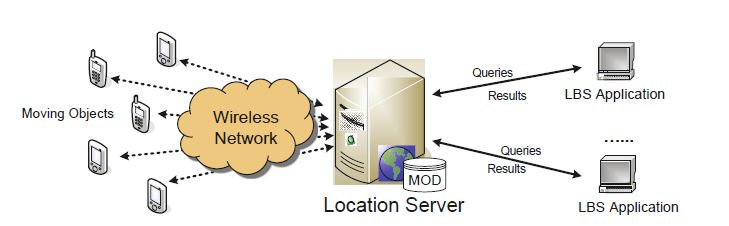
\includegraphics[scale=0.6]{LocationServer.JPG}

\caption{System model for locations based services}
\label{fig:system_model_for_locations_based_services}
\end{figure}


There are several options presented by \cite{Lee2011} how one can do data reduction and filtering techniques on spatial trajectories and thereby reduce the amount of data saved. There is batch compression (offline) and online algorithms for data reduction. Batch compression do computation on a full set of location points and then transmits it to the location server. Online algorithms computes directly on online selective data. We have created prototypes  of an offline and online algorithm namely Douglas-Peucker (DP) and Sliding Window. The implementations are elaborated in section~\ref{sec:prototypes}. 

Figure \ref{fig:douglas_peucker_algorithm} illustrates how DP using perpendicular Euclidian distance as the error measure together with a approximated trajectory (dotted line) and the original trajectory. If the error measure doesn't meet the threshold ($p_9$) a split point is created at ($p_9$). This results in a trajectory $p_0,p_9,p_{16}$. This process is repeated until the error measure between the approximated trajectory and the original trajectory is below the error threshold. The algorithm proceeds until all the location points in the original trajectory are visited.   

\begin{figure}[H]
\centering
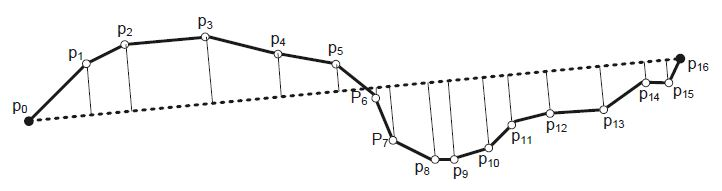
\includegraphics[scale=0.6]{DP.JPG}
\caption{Douglas-Peucker offline algorithm}
\label{fig:douglas_peucker_algorithm}
\end{figure}


The idea behind sliding window is to fit locations points in a growing sliding window with a valid line segment. The window continue to grow until approximation error threshold exceeds. The algorithm initializes the first location point of a trajectory as the anchor point $p_a$ of the window. The window slides when a new location point $p_i$ is added. As long all points within the sliding window doesn't exceeds the error threshold against a line segment new points are added. If the error threshold is violated the $p_{i-1}$ is included as part of the approximated trajectory and the $p_i$ is set to be the new anchor point $p_a$. An example of the sliding window is illustrated in figure \ref{fig:sliding_window_algorithm}. First the anchor point is set to $p_0$. The window slides \{$p_0,p_1,p_2,p_3,p_4$\} until $p_4$ is processed. Because the error threshold is violated for some location point within the sliding window, $p_3$ is included as a part of the approximated trajectory. The new anchor point $p_a$ is set to $p_3$.       
\begin{figure}[H]
\centering
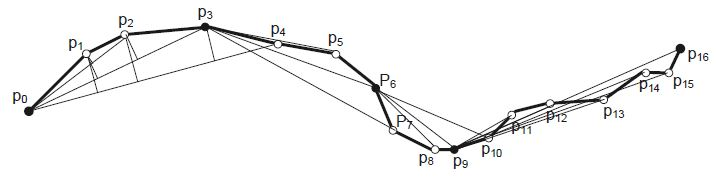
\includegraphics[scale=0.6]{SlidingWindow.JPG}

\caption{Sliding Window online algorithm}
\label{fig:sliding_window_algorithm}
\end{figure}


An alternative to sliding window is the open window algorithm. It is similar to the sliding window excepts when the error threshold is violated. The algorithm chooses the location point with the largest error distance as a part of the approximate trajectory whereas the sliding window included $p_{i-1}$ location point. This algorithm result in more accuracy compared to sliding window. 

\begin{figure}[H]
\centering
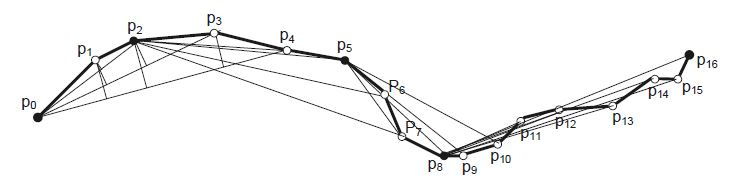
\includegraphics[scale=0.6]{OpenWindow.JPG}

\caption{Open Window online algorithm}
\label{fig:open_window_algorithm}
\end{figure}

These compressions algorithms suffers under location points which are potentially outliers. The compression isn't able to distinguish between "good" and "bad" points. One way to handle this is by applying a median filter. 

\iffalse
Suggestions for further processing:
\begin{itemize}
    \item Median filtering
    \item Advanced statistics calculations (analyse per interval)
    \item Algorithm to balance the trade-off between processing space and time (Appendix \ref{app:processing_algorithm})
\end{itemize}
\fi

\section{Closing the Sensing Loop}
% TODO:
% Apply definitions
% Little introduction
% Explain concepts
%    - Sharing
%    - Privacy 
%    - Personalization
% Relate to articles
% Relate to app: 
%    - privacy: delete raw data after processing
% Reflect and discuss
Closing the sensing loop deals with the final step of the continuous sensing where the collected and processed data is used to create value for the end user.
This is typically done by sharing the data either individually, with a group or for the community. 
Closing the sensing loop in our application happens after a bikebus has finished, where the data collection stops and the data is processed. Currently the newly processed statistics are added to the personal statistics for each user. These statistics will present the development of the user's cycling statistics.

Another idea for closing the sensing loop is to share the data with the municipality to gain better insight in people's cycling routines. This can benefit the community by detecting bottlenecks on bike paths (i.e. caused by poor traffic lighting or poor road construction) or missing bike parking in the city etc. 
The current application with individual sensing now becomes community sensing based instead.

When expanding the data sharing to the community the issue of privacy needs to be addressed. Location coordinates can be very sensitive private data and should be anonymous before sharing with the community.  

Ideas for applying privacy:
\begin{itemize}
    \item Share only the location and timestamp data and let the server assign the data a auto-generated primary key for the database. This makes all data independent from each other and the user.
    \item Share the data as batch file once a day to minimize live monitoring each user. Even though the location data is not connected to a specific person, it can be invasive to know that a person is at a specific place at the given moment.
\end{itemize}

In the article \cite{Mun2009} three different privacy countermeasures have been identified, which might be helpful to create more anonymous location data:
\begin{itemize}
    \item Selective Hiding: Generate location traces based on historical data to hide the actual data
    \item Spatial Routing: Use more coarse location data to blur out the fine location data
    \item Noise Addition: There is generated some noise of a location coordinate based on statistical distributions to be added to the coordinate
\end{itemize}

Of course there is a trade-off between the privacy and accuracy of the location data, which may be adjusted according the size of privacy needs and location accuracy. For instance when monitoring traffic data, the countermeasures should still be able to show which roads are used, else the data is not beneficial for traffic analysis.

        
%***************************************************************
%               Part 2: Architecture
%***************************************************************

\chapter{Architecture Qualities}
    % Sune
%TODO:
% Apply defintiions
% Short introduction to Architecture qualities
As software engineers our focus is on creating a software architecture based on the architectural requirements. Software architecture allows us to reasons and take qualified decision. It is essential that we early in the project    \cite{un}

\section{Quality Attributes}
We will follow the definition on software architecture from \cite{Bass}. 
%**************************************Definition Software architecture
\begin{defi}[\textbf{Software architecture}]
The software architecture of a system is the set of \textbf{structures} needed to reason about the system, which comprise software \textbf{elements}, \textbf{relations} among them, and the \textbf{properties} of both. 
\end{defi}
%**************************************Definition Software architecture End


Our approach towards implementing a software architecture is based on Quality attribute (QA) and Quality attribute scenario (QAS). A quality attribute (QA) according to \cite{Bass} is as follows.

%**************************************Definition Quality attribute
\begin{defi}[\textbf{Quality attribute}]
..A quality attribute is a measurable or testable property of a system that is used to indicate how well the satisfies the needs of its stakeholders..  
\end{defi}
%**************************************Definition Quality attribute End


% TODO:
% Introduction to QA
% List relevant quality attributes
% Why these attributes?
% Relate to generel mobile application challenges and tactics

From \cite{Bass} we have seven quality attributes here among modifiability, availability and performance. Furthermore \cite{Kjaergaard:2015:AQT:2737182.2737196} has added energy efficiency and and ressources adaptability.  


We will discuss different tactics on software architecture for achieving the business goal for the electronic voting application. A tactic according to \cite{Bass} is defined as.

%**************************************Definition Tactic
\begin{defi}[\textbf{Tactic}]
Tactic is a design decision that influences the achievement of a quality attribute response. 
\end{defi}
%**************************************Definition Tactic End

\section{Quality Attribute Scenarios}
% TODO:
% Formal definition of QAS
% Use template from Bass

A core observation is that a QA should be measurable or testable quality. The key point is when working with QA we use them in a given context/scenario and therefor we informally call these as QAS.\\



\begin{figure}[H]
\centering
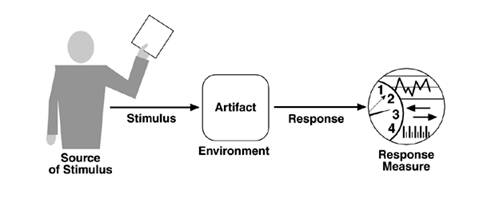
\includegraphics[scale=0.8]{QualityAttributeScenario.jpg}

\caption{The parts of a quality attribute scenario}
\label{fig:Quality_Attribute_Scenario}
\end{figure}






One of the core aspects of the definition of software architecture, is that software architecture is a set of structures, which we can use to reason about the system. To assist and visualize these structures, elements, relations and properties we use Module-, Component \& Connector (C\&C)- and Allocation viewpoints \cite{3+1}. 

\begin{enumerate}
    \item Module viewpoint is concerned with how functionality of the system maps to static development units. The focus will be on elements such as classes and interfaces and relationships such as associations, generalizations, realizations and dependencies.
    \item Component \& Connector viewpoint is concerned with the runtime mapping of functionality to components of the architecture. Components are the executing things that perform a function. Connectors are the communication channels between components. The purpose is to focus on the flow of data and responsibilities such as a network call or method call etc.
    \item Allocation viewpoint is concerned with how software entities are mapped to environmental entities. Here the focus are on the physical stuff such as computer or a network. We specify the environment in order to make the software running. 
\end{enumerate}


These viewpoint originates from $3+1$ article \cite{3+1}, where the $+1$ is the architectural requirements. These architectural requirements can be formulated through QAS.


In the following we formulated a modifiability, a energy efficiency and a ressource adaptablity QAS for the Bikebus application. We chose to focus on modifiability because we want the application to be easily modifiable when new changes has to be made. We chose to' focus on energy efficiency because we have limited battery available on the phone. We chose to focus on resource adaptability because the app is depended on network resources.

\begin{table}[H]
\begin{center}
\begin{tabular}{|p{0.3cm}|p{2.5cm}|p{8cm}|}
  \hline
  \multicolumn{2}{|p{3cm}|}{\bfseries Scenario(s):} & \#  1: A developer should be able to replace sensor frameworks during runtime and apply the changes within 30 minutes. \\
  \hline
  \multicolumn{2}{|p{3cm}|}{\bfseries Relevant Quality Attributes:} & Modifiability\\
  \hline
  \multirow{6}{*}{\begin{sideways}{\bfseries Scenario Parts}\end{sideways}}
  & {\bfseries Source:} & Developer \\
  \cline{2-3}
  & {\bfseries Stimulus:} & Needs to replace a sensor frameworks \\
  \cline{2-3}
  & {\bfseries Artifact} &  Code \\
  \cline{2-3}
  & {\bfseries Environment:} &  Design time \\
  \cline{2-3}
  & {\bfseries Response:} &  Replacement made and Unit tested\\
  \cline{2-3}
  & {\bfseries Response Measure:} & In three hours\\
  \hline
\end{tabular}
\caption{Modifiability QAS}
\end{center}
\end{table}



\begin{table}[H]
\begin{center}
\begin{tabular}{|p{0.3cm}|p{2.5cm}|p{8cm}|}
  \hline
  \multicolumn{2}{|p{3cm}|}{\bfseries Scenario(s):} & \#  2: 100  events arrives periodically to the Bikebus application with high energy availability for the application to process with an energy consumption of  XX watt per event. \\
  \hline
  \multicolumn{2}{|p{3cm}|}{\bfseries Relevant Quality Attributes:} & Energy efficiency\\
  \hline
  \multirow{6}{*}{\begin{sideways}{\bfseries Scenario Parts}\end{sideways}}
  & {\bfseries Source:} & 100 events \\
  \cline{2-3}
  & {\bfseries Stimulus:} & Arrives periodically \\
  \cline{2-3}
  & {\bfseries Artifact} &  Bikebus application \\
  \cline{2-3}
  & {\bfseries Environment:} &  High energy availability \\
  \cline{2-3}
  & {\bfseries Response:} &  Process data\\
  \cline{2-3}
  & {\bfseries Response Measure:} & Energy consumption of xx watt per event \\
  \hline
\end{tabular}
\caption{Energi efficiency QAS}
\end{center}
\end{table}




\begin{table}[H]
\begin{center}
\begin{tabular}{|p{0.3cm}|p{2.5cm}|p{8cm}|}
  \hline
  \multicolumn{2}{|p{3cm}|}{\bfseries Scenario(s):} & \#  3: When the network coverage disappears from the phone, the BikeBus application has fewer resources available and changes the level of service by initiating participatory sensing and degrading the average accuracy level to 80\%. \\
  \hline
  \multicolumn{2}{|p{3cm}|}{\bfseries Relevant Quality Attributes:} & Resource Adaptability\\
  \hline
  \multirow{6}{*}{\begin{sideways}{\bfseries Scenario Parts}\end{sideways}}
  & {\bfseries Source:} & Changes in network signal \\
  \cline{2-3}
  & {\bfseries Stimulus:} & No network coverage  \\
  \cline{2-3}
  & {\bfseries Artifact} &  BikeBus \\
  \cline{2-3}
  & {\bfseries Environment:} &  Few resources \\
  \cline{2-3}
  & {\bfseries Response:} &  Change level of service to participatory sensing\\
  \cline{2-3}
  & {\bfseries Response Measure:} & Degraded service level with an accuracy on average of 80\%\\
  \hline
\end{tabular}
\caption{Resource Adaptability QAS}
\end{center}
\end{table}


\section{Tactics}
% TODO:
% For each QA find tactics
% Examples
%   - Performance: Limit sampling rate
%       - Possible solution: Our hierarachy divide and 
%         conquer
%   - Modifiability: Encapsulation/coupling/cohesion
%       - Possible solution: Interfaces, multiple APIs 
%         and storage
%   - Availability: Redundancy (caching layer)
%       - Possible solution: local caching

\subsection{Modifiability}

\subsection{Energy Efficiency}
To fulfill the energy efficiency QAS the sensor replacement tactic is chosen to improve the energy consumption of  the application.
% keywords:
% - Use one sensor to decide if the location sensor should be used
% - Discussion about which sensor should decide if the location sensor should be used
%    - Activity Recognition: Might be more expensive than location itself but has high accuracy
%    - Significant motion sensor: Very low energy consumption, but does not check for biking (assume we are biking when collecting on a bikebus)
% - If there was a qas for accuracy this could be prototyped and tested, but if both activity rec and significant comply with the qas then there is no problem

%Evt: performance test with battery historian

\subsection{Resource Adaptability}
One tactic to fulfill response measure is resource selection. There will be a selection between the activity recognition together with location and the accelerometer. 

 
    


\chapter{Solution Approach}
    %Anna

% Domain layer 
% Data layer (firebase)
% tactics
%  - interfaces and listeners (dependecy injection) (composite pattern?)
%  - activity recognition vs significant
%  - No Location - new model for calculations
% choice of tecnhologies and sensors

\section{Application Architecture}



\section{Continuous Sensing Architecture}

The continuous sensing in this application is formed from the notions of:
\begin{itemize}
    \item Geofence 
    \item Location 
    \item Activity Recognition
\end{itemize}

When the user creates or applies to a bikebus two Geofences are created for the start and end destination on the route. When the user is within the one of the Geofences, the Geofence fires an event which either initiates or stops the data collection.
Concretely the application holds a SensorDataController, which controls the flow of sensor data. 
\begin{enumerate}
    \item Creating two Geofence pending intents from the GoogleGeofence class
    \item The GeofenceIntentService class receives a GoogleGeofenceEvent object when a Geofence is triggered
    \item Based on the information from the Geofence event the GeofenceIntentService sends a status and result value back to the SensorDataController through a BroadcastReceiver
    \item The SensorDataController either stops the activity recognition or creates pending intents at a given sample rate from the GoogleActivityRecognition class
    \item Each time the ActivityRecognizeService class receives an intent with a ActivityRecognitionResult object the intent service broadcasts the results back to the SensorDataController
    \item Based on the activity has the value "ON\_BICYCLE" the SensorDataController will retrieve the current location of the user and store all locations for data processing
\end{enumerate}

\begin{figure}[H]
\centering
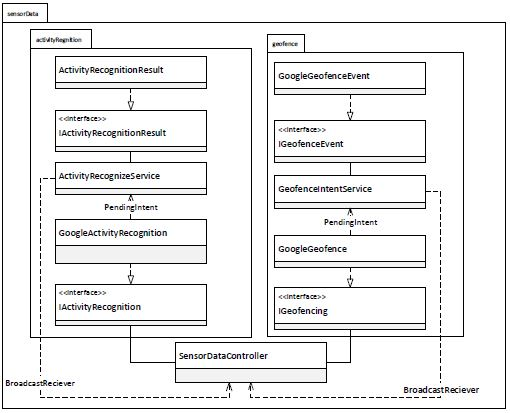
\includegraphics[scale=1]{Graphics/Images/Module_View_SensorData.jpg}
\caption{Module view of sensorData package}
\label{fig:Module_View_Sensor_Data}
\end{figure}
In figure \ref{fig:Module_View_Sensor_Data} a module view has been created based on the continuous data collection description. 

In Android there is typically two methods to apply when wanting to create background processes:
\begin{itemize}
    \item IntentService
    \item AsyncTask
\end{itemize}

The IntentService is a method used for long-term running background processes that is not dependent on the Activity. The AsyncTask is oppositely a method that only exists in the Activity's lifecycle, because it needs to return the value directly to the Activity. Therefore the AsyncTask cannot continue to run outside the application, and is more suited for short-term running background processes which are dependent on the Activity. 
\footnote{\url{https://github.com/codepath/android_guides/wiki/Starting-Background-Services}}

\section{Graphical User Interface}
The graphical design of this application is strongly inspired from another app called "GoMore", which has the concept of coordinating carpools. The "GoMore" concept reminds a lot about the "BikeBus" concept, because both apps coordinates for friends and strangers to ride with each other. The main differences between the two concepts are that "BikeBus" coordinates free bicycle rides and paid "GoMore" coordinates Car rides.

\begin{figure}
    \centering
    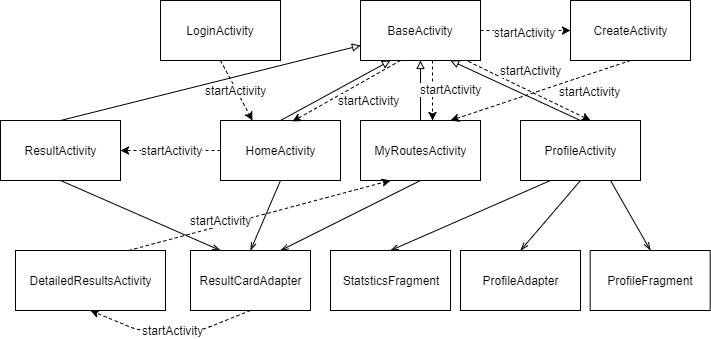
\includegraphics[scale=0.5]{Graphics/Images/Activity_Diagram.png}
    \caption{Diagram of activities}
    \label{fig:my_label}
\end{figure}

%% MISSING DESCRIPTION OF ACTIVITY DIAGRAM%%

\subsection{Design}
The "BikeBus" application follows the "Material Design" principles created by Google\footnote{\url{https://material.io/guidelines/#}}, which are quite popular for Android apps. Material Design has great guidelines on how to improve mobile user experience and can quickly make the application look more professional.

The Android GUI components used to provide the Material Design elements:
\begin{itemize}
    \item CardView - The card element containing information of the bikebus
    \item RecyclerView - Infinity scroll view containing only cardviews
    \item BottomNavigationView - The bottom navigation menu between search, routes and profile tabs
    \item TabLayout with ViewPager - A Tab view in the profile view which switches between the profile and statistics fragment
    \item FloatingActionButton - The red create button
\end{itemize}

In this project Google API's has been frequently used for especially sensor data, but the Google AutoComplete

\begin{figure}[!htb]
\centering
\begin{minipage}{0.32\textwidth}
\centering
    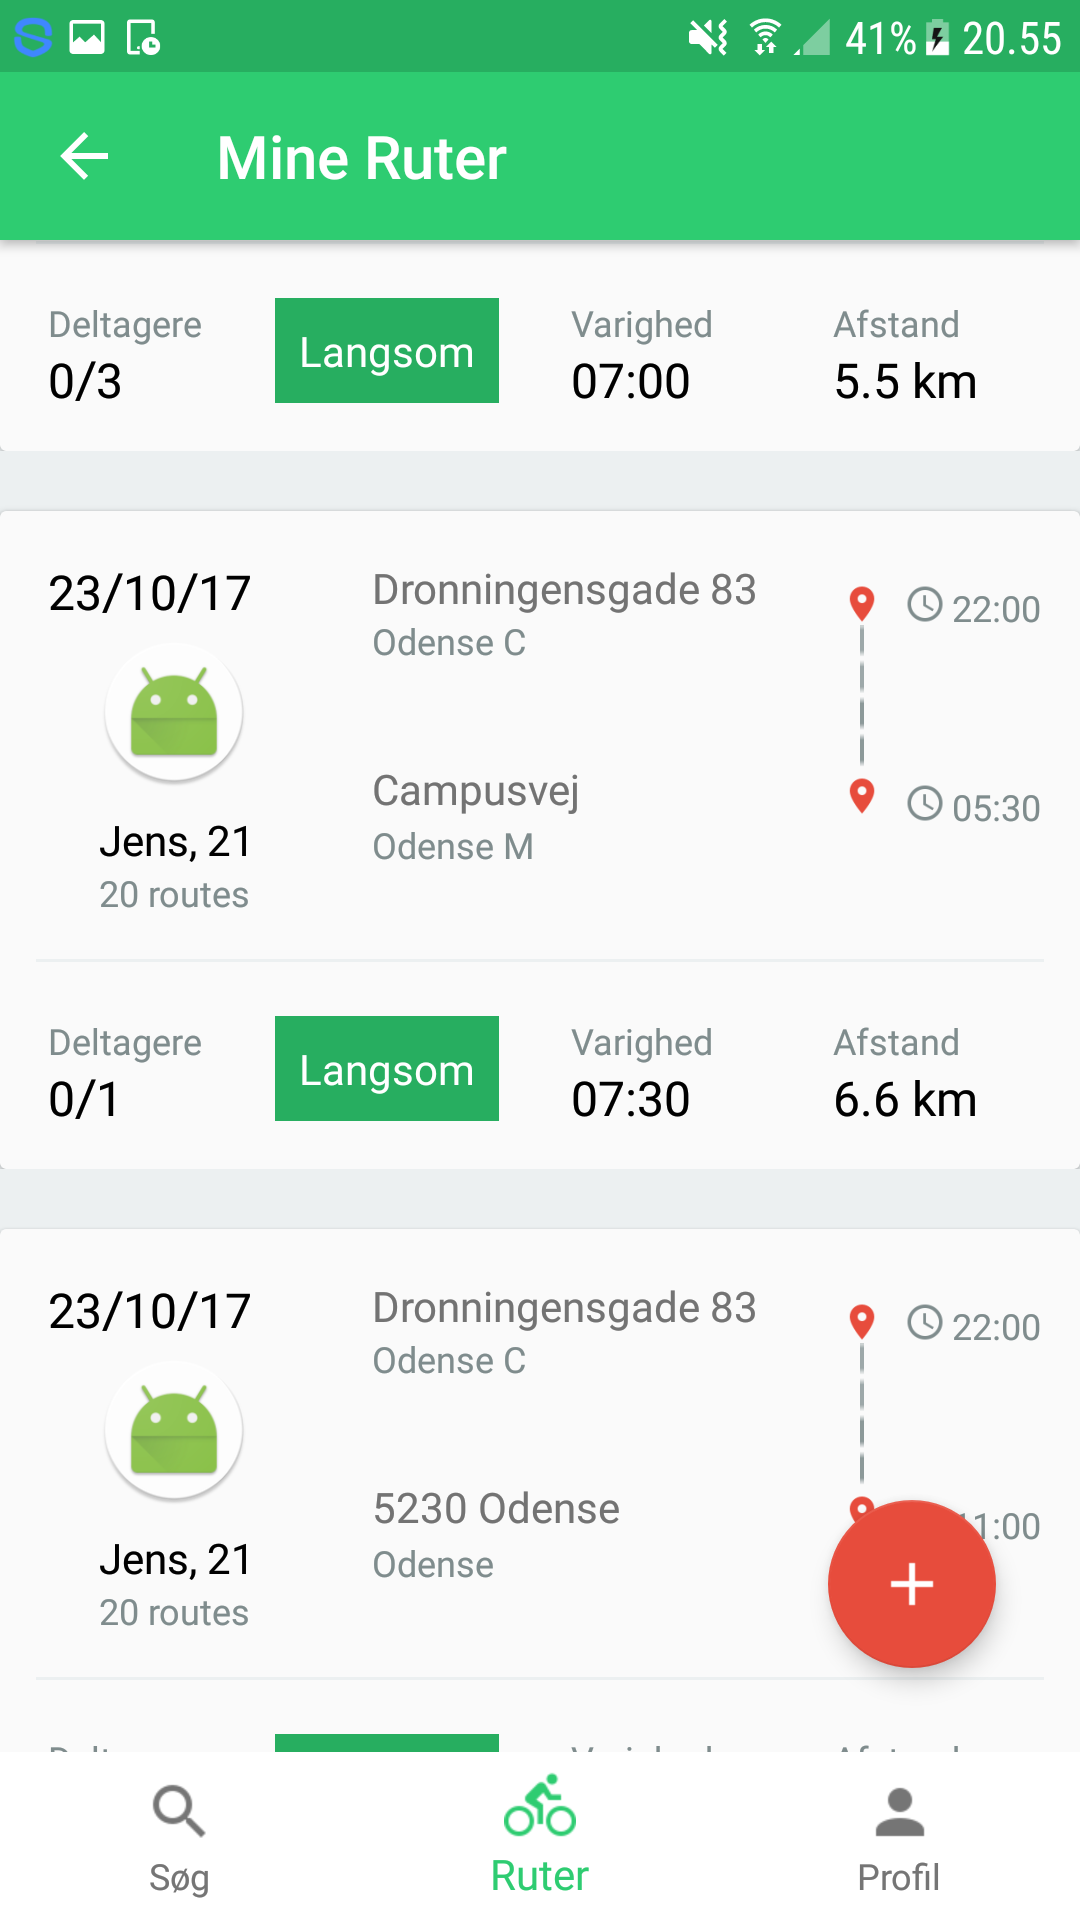
\includegraphics[width=\linewidth]{Graphics/Images/bikebus_search.png}
    \caption{Result page for BikeBus}
    \label{fig:sample_figure}
\end{minipage}\hfill
\begin{minipage}{0.32\textwidth}
\centering
    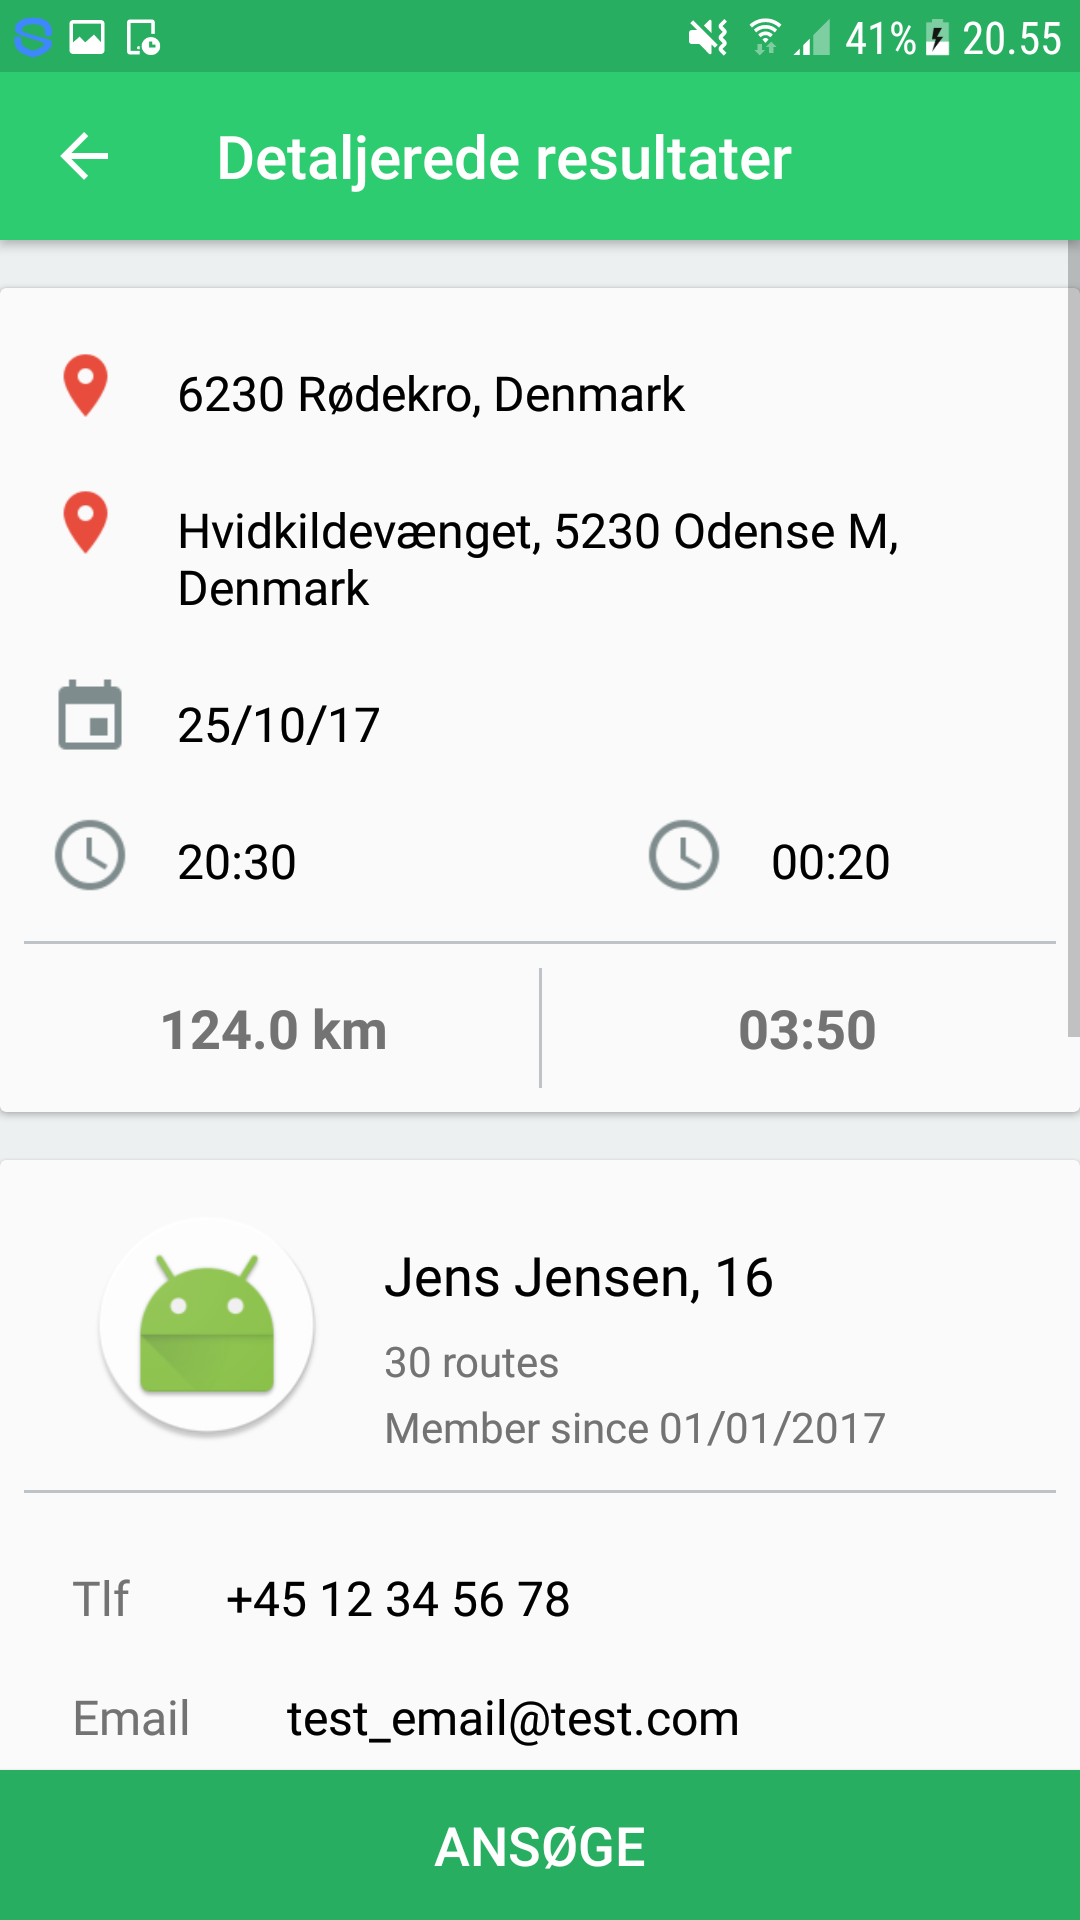
\includegraphics[width=\linewidth]{Graphics/Images/bikebus_detail_1.png}
    \caption{Detailed page for BikeBus (part 1)}
    \label{fig:sample_figure}
\end{minipage}\hfill
\begin{minipage}{0.32\textwidth}
\centering
    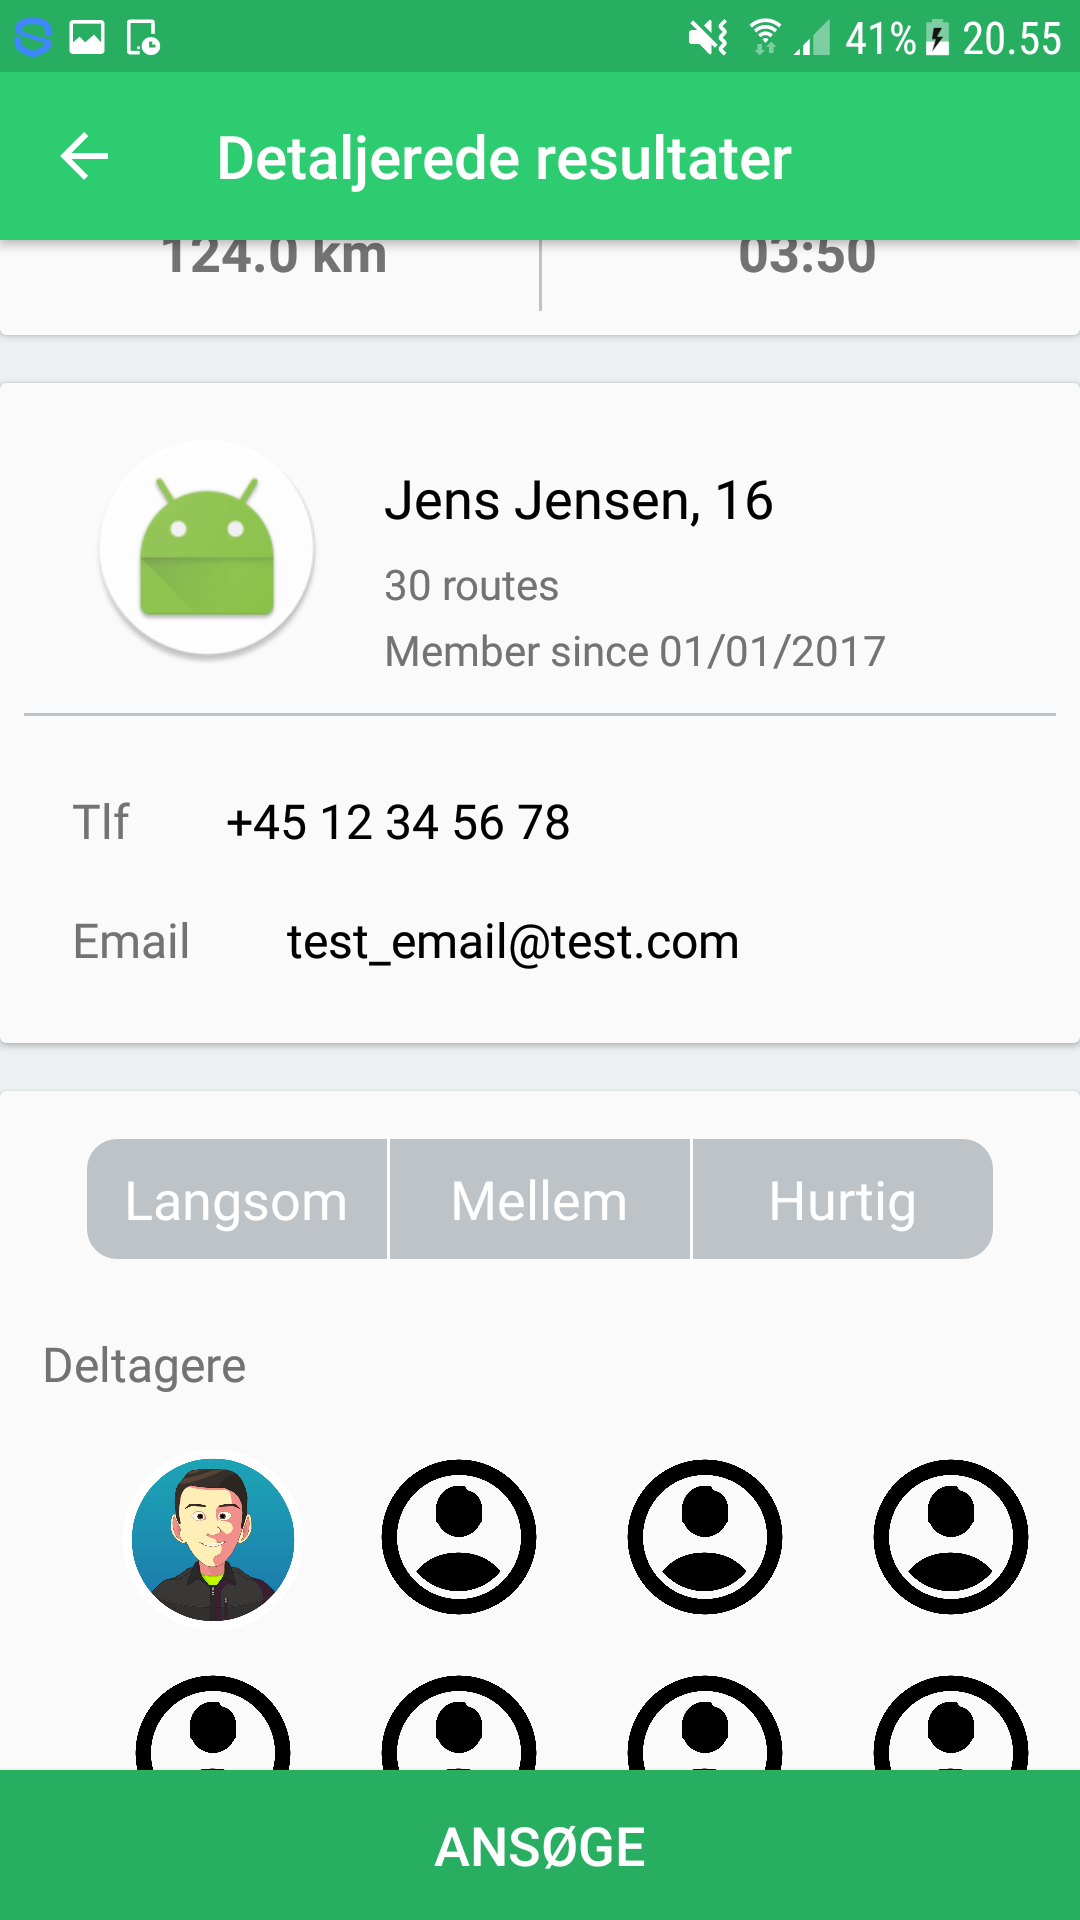
\includegraphics[width=\linewidth]{Graphics/Images/bikebus_detail_2.png}
    \caption{Detailed page for BikeBus (part 2)}
    \label{fig:sample_figure}
\end{minipage}
\end{figure}

\chapter{Solution Description}
    % Admir, Anna,  Sune (prototype)

% API implementation - Google, Firebase, Activity Recognition (Admir)
% Data Collection - Geofence, Activity Recognition, Location (Sune)
% Search (Sune)
% Distance calculator
% ILocation and IStorage or other with interface and listener
% Adapter view pattern (Anna)

% TODO:
% Apply definitions
% Introduction
% Explain three different categories of prototyping
%    - Explorative, Experimental, Evoulutionary

\section{Prototypes}
\label{sec:prototypes}

% TODO:
% Explain all protoypes in our program (Implementation)
%    - Datastructures, algorithms, storage, etc
%    - Diagrams
%    - Results of prototypes

% Current Prototypes:
% - Easily shift sensor API (modifiability) 
%    - EmotionSenseLocation.java and ILocation  
% - SQLite for internal storage (availablity)


% Prototypes:



%***************************************************************
%               Part 8: Related work
%***************************************************************
\chapter{Related Work}
    % Admir

% TODO:
% Collect all articles 
% Describe related apps (GoMore, CykelScore, ...)
% UX material design
% Other resources
%***************************************************************
%               Part 9: Reflection 
%***************************************************************
\chapter{Reflection and Discussion}
    %(All)

% TODO:
% Overall evaulation and discussion
%***************************************************************
%               Part 9: Conclusion
%***************************************************************
\chapter{Conclusion}
    % Conclusion (All)
% Future Work (Admir)

% TODO:
% Conclusion, Perspective, Future Work

%***************************************************************
%               Bibliography
%***************************************************************
\addcontentsline{toc}{chapter}{\\BIBLIOGRAPHY}
\bibliographystyle{alpha}
\bibliography{901_Bibliography}

\clearpage
%***************************************************************
%               Appendex
%***************************************************************
\appendix
\addcontentsline{toc}{chapter}{\\APPENDICES}
\chapter{Proofs}
\section{Assignment 1 images}

\label{app:confusion_matrix}
\begin{figure}[H]
\centering
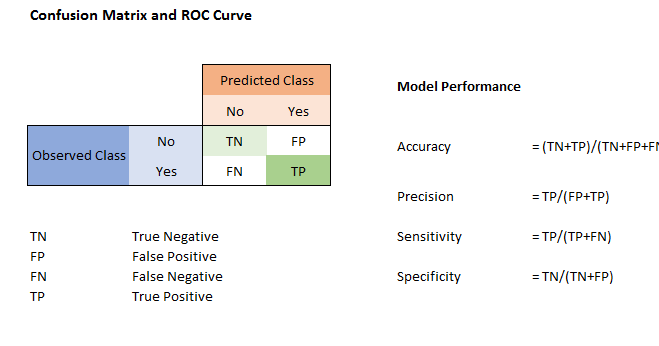
\includegraphics[scale=0.55]{Graphics/Assignment1/ConfusionMatrix.png}
\caption{Confusion Matrix}
\label{fig:confusion_Matrix}
\end{figure}

\subtitle{LDA coefficients results}
\begin{figure}[H]
\centering
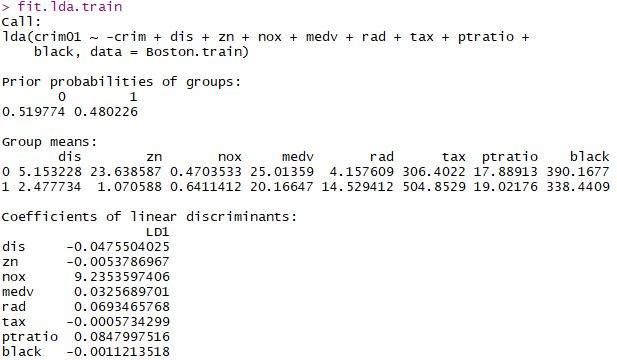
\includegraphics[scale=0.55]{Graphics/Assignment1/LDACoefficients_005.JPG}
\caption{Coefficients for significance level 5\%}
\label{fig:coefficients_method_005}
\end{figure}

\begin{figure}[H]
\centering
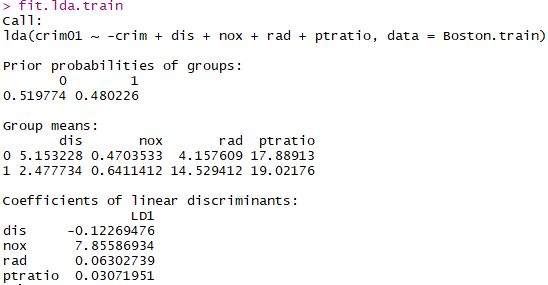
\includegraphics[scale=0.55]{Graphics/Assignment1/LDACoefficients_001.JPG}
\caption{Coefficients for significance level 1\%}
\label{fig:coefficients_method_001}
\end{figure}

\begin{figure}[H]
\centering
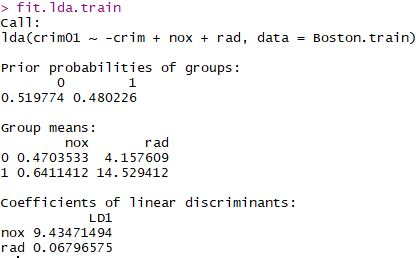
\includegraphics[scale=0.55]{Graphics/Assignment1/LDACoefficients_0001.JPG}
\caption{Coefficients for significance level 0.1\%}
\label{fig:coefficients_method_0001}
\end{figure}


\section{Assignment 3 images}
%--------------- Renoir Image -------------------------
\begin{figure}[H]
    \centering
    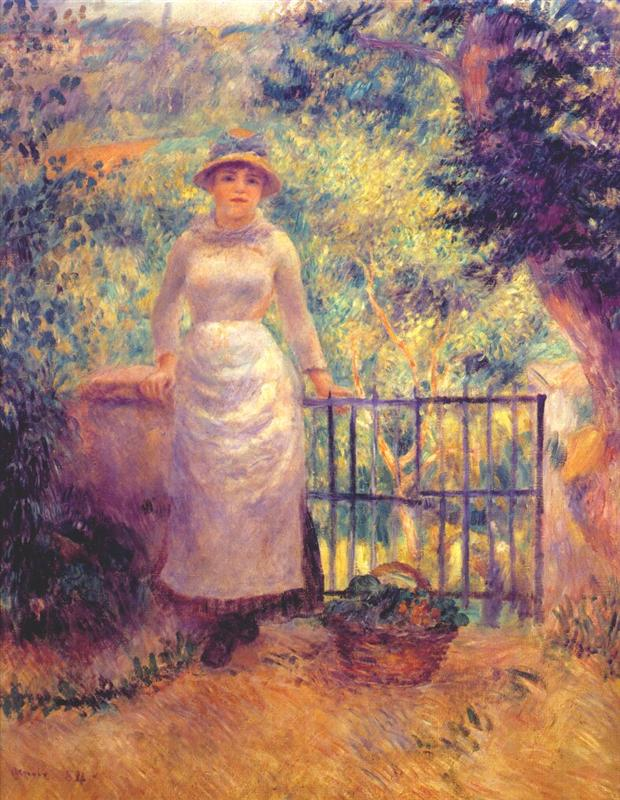
\includegraphics[scale=0.3]{Graphics/Assignment3/renoir.png}
    \caption{Pierre-Auguste Renoir: Aline at the gate.}
    \label{fig:renoir}
\end{figure}
%--------------- Outlier Image -------------------------

\begin{figure}[H]
    \centering
    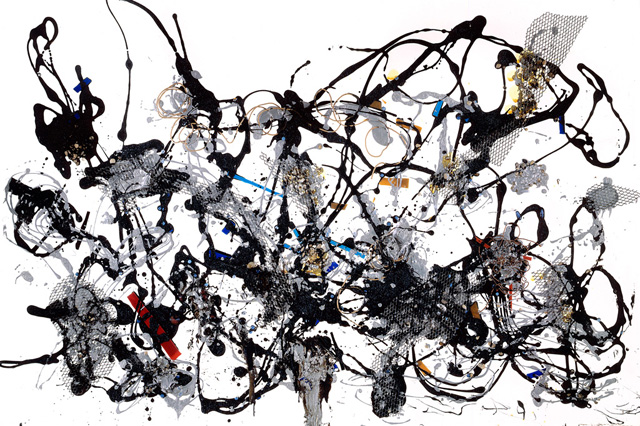
\includegraphics[scale=0.5]{Graphics/Assignment3/outlier.png}
    \caption{Jackson Pollock: Number 29.}
    \label{fig:outlier}
\end{figure}

%--------------- Manet Image -------------------------
\begin{figure}[H]
    \centering
    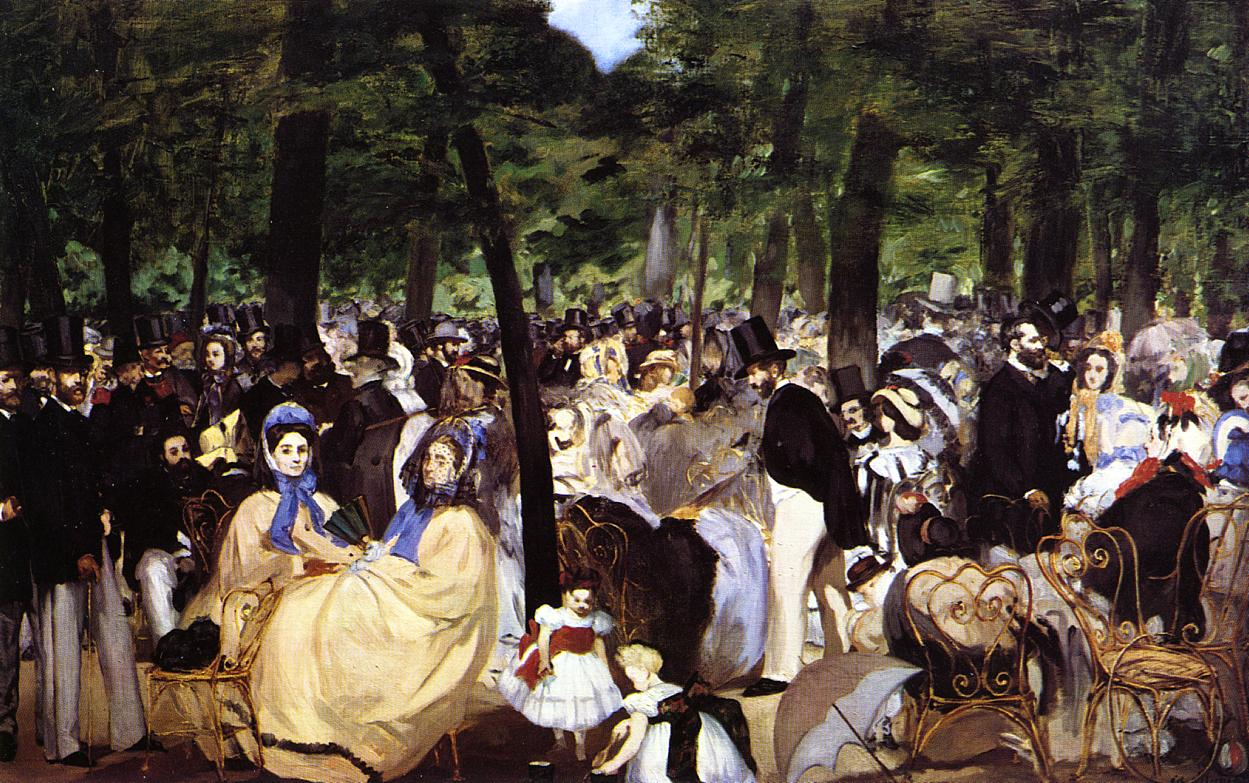
\includegraphics[scale=0.3]{Graphics/Assignment3/manet.png}
    \caption{Édouard Manet: Music in the Tuileries.}
    \label{fig:manet}
\end{figure}


%--------------- Degas Image -------------------------

\begin{figure}[H]
    \centering
    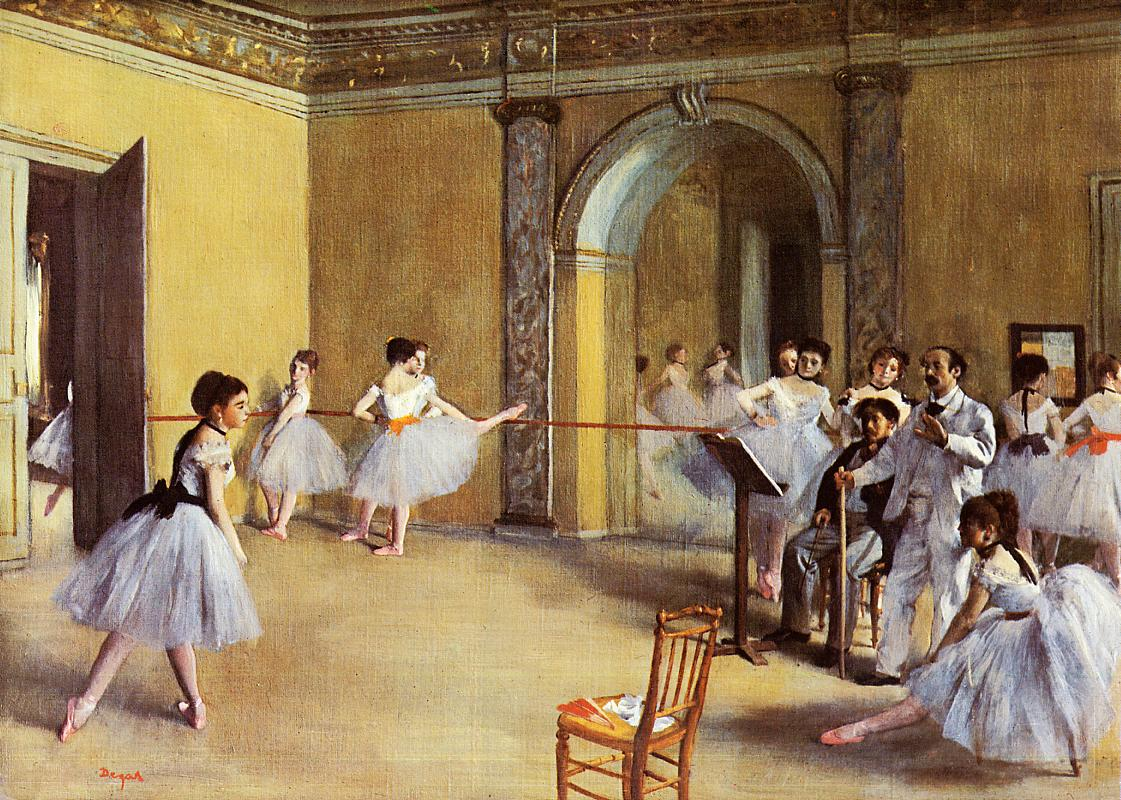
\includegraphics[scale=0.3]{Graphics/Assignment3/degas.png}
    \caption{Edgar Degas: Dance Class at the Opera.}
    \label{fig:degas}
\end{figure}

%--------------- VGG16 model Image -------------------------

\begin{figure}[H]
    \centering
    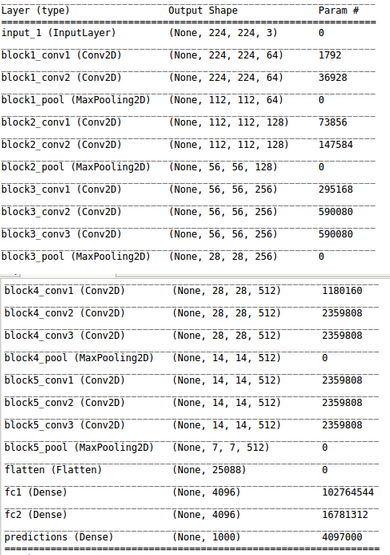
\includegraphics[scale=0.7]{Graphics/Assignment3/VGG16_model_image.png}
    \caption{VGG16 model with 1000 classes as output.}
    \label{fig:imagenet_vgg16}
\end{figure}

%--------------- Custom VGG16 model Image -------------------------

\begin{figure}[H]
    \centering
    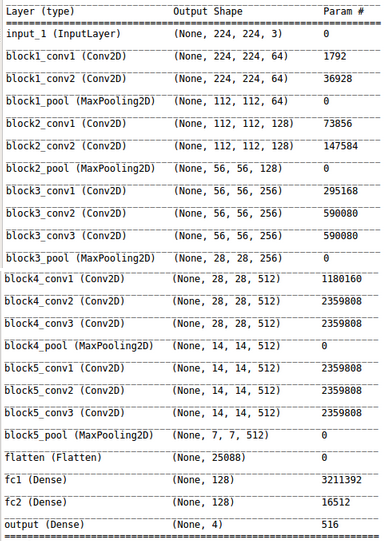
\includegraphics[scale=0.7]{Graphics/Assignment3/custom_model_image.png}
    \caption{Custom VGG16 model with 4 classes as output.}
    \label{fig:custom_vgg16}
\end{figure}

\section{Assignment 3 code}

%------------------ Fetch image code ----------------------
\begin{lstlisting}[frame=single, language=Bash, label={code:fetch_images}, caption={Code to fetch images from Wikiart for specific artists, in this case Manet.}]
    curl -s "https://www.wikiart.org/en/App/Painting/PaintingsByArtist?artistUrl=edouard-manet&json=2" | jq -r 'map(.image) | join("\n")' | sed '' | xargs -P 10 -n 1 curl -s -O
\end{lstlisting}

%------------------ Load data for preprocessing ---------------
\begin{lstlisting}[frame=single, language=Python, label={code:load_data}, caption={Code to load data for preprocessing.}]
    for dataset in data_dir_list:
	    img_list=os.listdir(data_path+'/'+ dataset)
    	for img in img_list:
    		img_path = data_path + '/'+ dataset + '/'+ img 
    		img = image.load_img(img_path, target_size=(224, 224))
    		x = image.img_to_array(img)
    		x = np.expand_dims(x, axis=0)
    		x = preprocess_input(x)
    		img_data_list.append(x)
\end{lstlisting}


%------------------- Shuffle and split into training and test --------------------
\begin{lstlisting}[frame=single, language=Python, label={code:shuffle_and_split_data}, caption={Code to shuffle and split the data to 80\% training and 20\% test.}]
#Shuffle the dataset
x,y = shuffle(img_data,Y, random_state=2)

# Split the dataset
X_train, X_test, y_train, y_test = train_test_split(x, y, test_size=0.2, random_state=2)
\end{lstlisting}

\begin{lstlisting}[frame=single, language=Python, label={code:model_creation_and_training}, caption={Code to load VGG16 pre-trained on ImageNet and doing transfer learning.}]
# Adjust the image input to 224, 224 and 3 channels
image_input = Input(shape=(224, 224, 3))

# VGG16 model
model = VGG16(input_tensor=image_input, include_top=True,weights='imagenet')

# Get VGG16's block5_pool layer and take its output
last_layer = model.get_layer('block5_pool').output
# Feed the output of block5_pool to the Flatten layer
x= Flatten(name='flatten')(last_layer)
# Create two fully connected layers with 128 neurons each, using RELU activation
x = Dense(128, activation='relu', name='fc1')(x)
x = Dense(128, activation='relu', name='fc2')(x)
# Create a output layer, using softmax classification
out = Dense(num_classes, activation='softmax', name='output')(x)
# Assign the new model to a variable
custom_vgg_model2 = Model(image_input, out)

# Freeze all the layers except the dense layers that was created above
for layer in custom_vgg_model2.layers[:-3]:
	layer.trainable = False

# Compile the new model architecture
custom_vgg_model2.compile(loss='categorical_crossentropy',optimizer='adadelta',metrics=['accuracy'])

# Time it
t=time.time()
# Train the model for 20 epochs using a batch size of 4
hist = custom_vgg_model2.fit(X_train, y_train, batch_size=4, epochs=20, verbose=1, validation_data=(X_test, y_test))
print('Training time: %s' % (t - time.time()))
# Test the model using accuracy as a metric
(loss, accuracy) = custom_vgg_model2.evaluate(X_test, y_test, batch_size=10, verbose=1)
print("[INFO] loss={:.4f}, accuracy: {:.4f}%".format(loss,accuracy * 100))
\end{lstlisting}





\end{document}
